\documentclass[12pt]{article}  % [12pt] option for the benefit of aging markers
\usepackage{amssymb,amsthm}    % amssymb package contains more mathematical symbols
\usepackage{graphicx}          % graphicx package enables you to paste in graphics
\usepackage[capposition=top]{floatrow}
\usepackage{setspace}
\usepackage{float}
\usepackage[backend=bibtex,sorting=nyt,firstinits=true]{biblatex}
\usepackage{hyperref}
\usepackage{longtable}
\usepackage{wrapfig}
\usepackage[titletoc,title]{appendix}
\usepackage{pdfpages}
\usepackage{color, colortbl}

\usepackage{lipsum}
\usepackage[margin=2cm]{geometry}

\definecolor{Gray}{gray}{0.9}


\addbibresource{references.bib}
\newcommand{\rid}[1]{\centering #1-\ifnum\value{requirement}<10 0\fi\arabic{requirement} \stepcounter{requirement}}



%%%%%%%%%%%%%%%%%%%%%%%%%%%%%%%%%%%%%%%%%
%										%
%     			Title					%
%										%
%%%%%%%%%%%%%%%%%%%%%%%%%%%%%%%%%%%%%%%%%
\title{Digital Lab Marking System \\~\\  \large{Heriot-Watt University} \\~\\ Deliverable 1: Final Year Dissertation \\~\\ MEng Software Engineering}
\author{Lewis Francis McNeill\\
supervised by
Peter J King}

\begin{document}
\maketitle
\pagenumbering{gobble}



%%%%%%%%%%%%%%%%%%%%%%%%%%%%%%%%%%%%%%%%%
%										%
%     		    Declaration				%
%										%
%%%%%%%%%%%%%%%%%%%%%%%%%%%%%%%%%%%%%%%%%
\newpage
\setcounter{page}{1}
\pagenumbering{roman}
\doublespacing
\textbf{\Large{Declaration}} \\[2em]
I, Lewis Francis McNeill, confirm that this work submitted for assessment is my own and is expressed in my own words. Any references, made within it, of the works of other authors in any way (e.g., ideas, equations, figures, text, tables, programs) are properly acknowledged at any point of their use. A list of the references employed is included.
\\
\\
Signed: Lewis McNeill
\\
Date: \today


%%%%%%%%%%%%%%%%%%%%%%%%%%%%%%%%%%%%%%%%%
%										%
%     		    Abstract				%
%										%
%%%%%%%%%%%%%%%%%%%%%%%%%%%%%%%%%%%%%%%%%
\newpage               
\begin{abstract}
\noindent
The aim of this dissertation project is to replace the current system for the marking of computer labs with a new digital system. This will enable lecturers to create a marking scheme online. Lab helpers will select the student they are marking and the marking scheme will then be loaded, marks will be entered and then made immediately available to both student and lecturers to view. It will also provide useful statistics for both student and lecturers.
\end{abstract}
\newpage                
\tableofcontents




%%%%%%%%%%%%%%%%%%%%%%%%%%%%%%%%%%%%%%%%%
%										%
%     		Introduction				%
%										%
%%%%%%%%%%%%%%%%%%%%%%%%%%%%%%%%%%%%%%%%%
\newpage   
\setcounter{page}{1}
\pagenumbering{arabic}
\section{Introduction}

The current system for marking of computing science labs is to use multiple lab helpers, each given a list of students and the marking scheme for them. Generally marking schemes are a selection of tasks students must have completed and lab helpers tick them off when this has been achieved. The biggest problem with this part of the marking is the length of time it takes lab helpers to locate the students on the list. This causes frustration with increased waiting times for students.  Multiple other issues  can also  arise from this: students can be marked by two helpers and obtain different grades from both; the lab helper omits to  tick off a completed task; they assign  marks for the wrong student on the sheet or simply they misplace the actual marking sheet.

After the lab helpers have completed their marking, the sheets are provided to the lecturer who collates them together into one spreadsheet to calculate marks. After that it is entered it into vision. This too can cause its own set of problems-the chances of transcription errors are increased as it is possible for the lecturer to misread marks when they are transferring them across. The lecturer may not enter the marks immediately into the spreadsheet increasing the chance that a marking sheet goes missing, and finally this system means that students are having to wait even longer to receive their results.

The objective is to develop a system that will reduce and hopefully eliminate the problems of the current system. Along with this, it should hopefully reduce the amount of time taken to mark students’ work and therefore speed up labs in general. It should also enable students to see their grades immediately, allow lecturer to see the result of the assignments as they are being marked and make marking quicker for lab helpers.




\newpage
\section{Aims and Objectives}
\subsection{Aim}
The aim of this dissertation is to design and implement a system for the digital marking and analysis of computer labs and to help improve the speed at which they are marked. The system will also provide useful statistics for both lecturers and students.

\subsection{Objectives}
\label{section:object}
\begin{itemize}
\item Simplify the way that labs marks are currently processed.
\item Allow lecturers to create marking schemes on-line that lab helpers can access. 
\item Lab helpers can mark students in labs using marking schemes.
\item Lab helpers able  to mark labs using an on-line application.
\item Allow students to see the mark they achieved from the lab instantly.
\item Provide useful statistics and graphs for lecturers and students.
\item Provide different views for student, lab helpers and lecturer.
\end{itemize}



%%%%%%%%%%%%%%%%%%%%%%%%%%%%%%%%%%%%%%%%%
%										%
%     	   Literature Review			%
%										%
%%%%%%%%%%%%%%%%%%%%%%%%%%%%%%%%%%%%%%%%%
\newpage
\section{Literature Review}
This section contains the summaries of literature relating to the topic and should help to create a context for the development of a digital marking system. It will cover what marking systems that are currently being used, what current digital marking systems actually exist and why they are an improvement. Along with this it will also cover how to control what users are allowed to see, as well as explaining systems for creation of custom website forms, and finally it will cover the graphical displaying of statistics. 


\subsection{Web Applications}

%TODO%


\subsection{Marking Systems}

\subsubsection{Lecturer Based}
The way lecturer based marking works is that students complete their assignment, the lecturer or tutor marks it and provides result in a timely manner with useful feedback which can be majorly important in helping students improve their skills  \cite{tang_investigating_2011}.

The advantage of this style of marking is that students can obtain useful feedback from their lecturer that can help improve their learning.  An article study \cite{higgins_conscientious_2002} found that of the students, when surveyed 82\% agreed to the question "I pay close attention to the comments I get" in response to assignment feedback.

A downside to this style of marking is that as the number of students increases on courses the amount of time required to mark assignments consequently takes longer and in some cases this can actually cause marked assessments to be scrapped completely due tomthemamount of time taken to give feedback to students \cite{brown_assessment_1999}.


\subsubsection{Peer Based}
To cope with increasing class sizes some courses are beginning to move towards peer marking. Peer marking system works by having students assess each other and in some cases  the students produced their own marking criteria \cite{orsmond_use_2000}.

This style allows  students to gain experience in evaluating other people's work, which some graduates feel is a necessary skill to possess. \cite{langan_insights_????}. Peer marking also deals with increasing amounts of students very well- this is because as the number of students increases the number of markers also increases!

Peer marking however has its own set of problems - for example, "Students may have a less well developed sense of the criteria compared to the lecturer which could lead to a lack of reliability of student marking." \cite{orsmond_use_2000}.



\subsection{Digital Marking Systems}

\subsubsection{Reasons for Digital Marking}
Digital marking systems are designed to mirror the current paper based marking systems but with the advantage of the electronic environment \cite{heinrich_online_2003}. These systems help to reduce the increasing workload caused by more and more students taking courses. Along with this it also allows administrative tasks associated with coursework to be automated enabling more time for other tasks.\cite{joy_effective_1998}.

For students digital marking is great as it allows for quick feedback as the assessor is able provide students feedback immediately after they have written it up, instead of having to wait for a class to receive it. In one study\cite{dahl_turnitin_2007} they found that 78\% of students would like get their feedback  electronically .

According to the highlighted article \cite{derby_duplication_2008} plagiarism is on the rise amongst student. This is where digital marking can help to reduce plagiarism as the programme can  do what a human marker cannot. They can compare a submission thousands of documents and judge if a person has plagiarised. They can also help to show patterns in assignments and marks that normally might go unnoticed.


\newpage
\subsubsection{TurnItIn}
There currently exists an on-line electronic plagiarism system called TurnItIn, \cite{_turnitin_????} currently being used by many universities around the world. It allows students to upload their essay assignments online. It then checks for plagiarism in the document by searching the internet and using a large database of documents. After it processes the document it assigns a plagiarism percentage and highlights any areas that were plagiarised. Lecturers can then login and view all the submitted documents and mark them .\\
Current research highlighted \cite{dahl_turnitin_2007} conducted a questionnaire and found that students felt that the system was easy to use and more convenient than having to provide paper copies. It also found that 50\% of students strongly agreed and 33.3\% just agreed that they preferred to have their grade shown online rather than have a cover sheet.

\subsubsection{BOSS System}
The BOSS system  was developed at the University of Warwick to help deal with their problem of having too many students for the number of staff and yet wanting students to have accurate and quickly available feedback \cite{joy_boss_2005}.
It is an electronic submission and assessment system created to allow computing science students to submit their programming assignments and have them tested and marked online \cite{joy_effective_1998}. The system is not designed to remove human markers completely, instead simply "assist the instructor in achieving a quicker, more accurate and more consistent assessment of programming assignment"\cite{joy_boss_2005}.

When a file is first submitted it is run through a plagiarism check to make sure that the submission is actually the student’s own work. It also checks that the submission passes pre-set tests to make sure it works. After this it goes into the evaluations stage, since evaluation attributes of code can be very subjective what the second step does is generate metrics about the submitted program. Some of these metric are a number of comments and percentage of methods declared \cite{joy_effective_1998}, which will help human markers evaluate the submission quicker.



\subsection{User Access Views}

\subsubsection{Social Media}
Controlling the view that users have, based on their access level, is common practice. Social media websites for instance allow users to limit what others  can see, through the use of a privacy setting \cite{tufekci_can_2008}. This means that another user's view is determined by the access level they are given for example, a user that is a friend will have a higher access and be allowed to see their whole feed, while an other users access may only allow them see the profile name.

\subsubsection{Database Controlled Access}
The patent highlighted \cite{baker_system_1997}, describes a system of limiting user web page access through the use of relation databases. The system would work by using two databases; one would hold a list of all the url's and associated access level, while the second database would hold all the user id's along with their assigned access level. When a user requests a webpage, the access level for that webpage and the user are looked up. If the users do not have the appropriate access they are denied permission to load the page and depending on implementation may be redirected to another webpage.
The design of this system is well suited for scalability since no matter how large the two datasets are only one piece of data is need from each database to confirm whether a user is allowed access.


\subsection{Custom Input Forms}

\subsubsection{SurveyMonkey}
Survey Monkey \cite{finley_surveymonkey_1999} is an example of custom web forms being created by users. Founded by Ryan Finley in 1999 Survey Monkey enables users to create their own surveys and easily distribute them. It builds the surveys by letting the user select the contents of the question and what the response type will be: The user can also decide if the responses are completely anonymous by default and the participants ip address is stored when they complete the survey. The users can continue to add as many questions as they would like, even after the survey is initially created. After designing the survey the user chooses how they would like to have their survey distributed. The available options that can be selected are a web link, social media, email or embeddable on a website \cite{waclawski_how_2012} .

When participants complete the survey their results are immediately stored and the results of the survey are visible to the user by login into their account on surveymonkey. They can choose to look at the responses individually or look at metrics about how participants responded.


\subsubsection{Customizing Forms In Electronic Mail Systems}
\noindent
A patent \cite{holt_customizing_2006} describes a process for user-customisable forms in an e-mail system where the administrator selects custom field types and behaviours.  For example current e-mail forms have

\begin{wrapfigure}[7]{r}{0.5\textwidth}
\vspace*{-\baselineskip}
\begin{figure}[H]
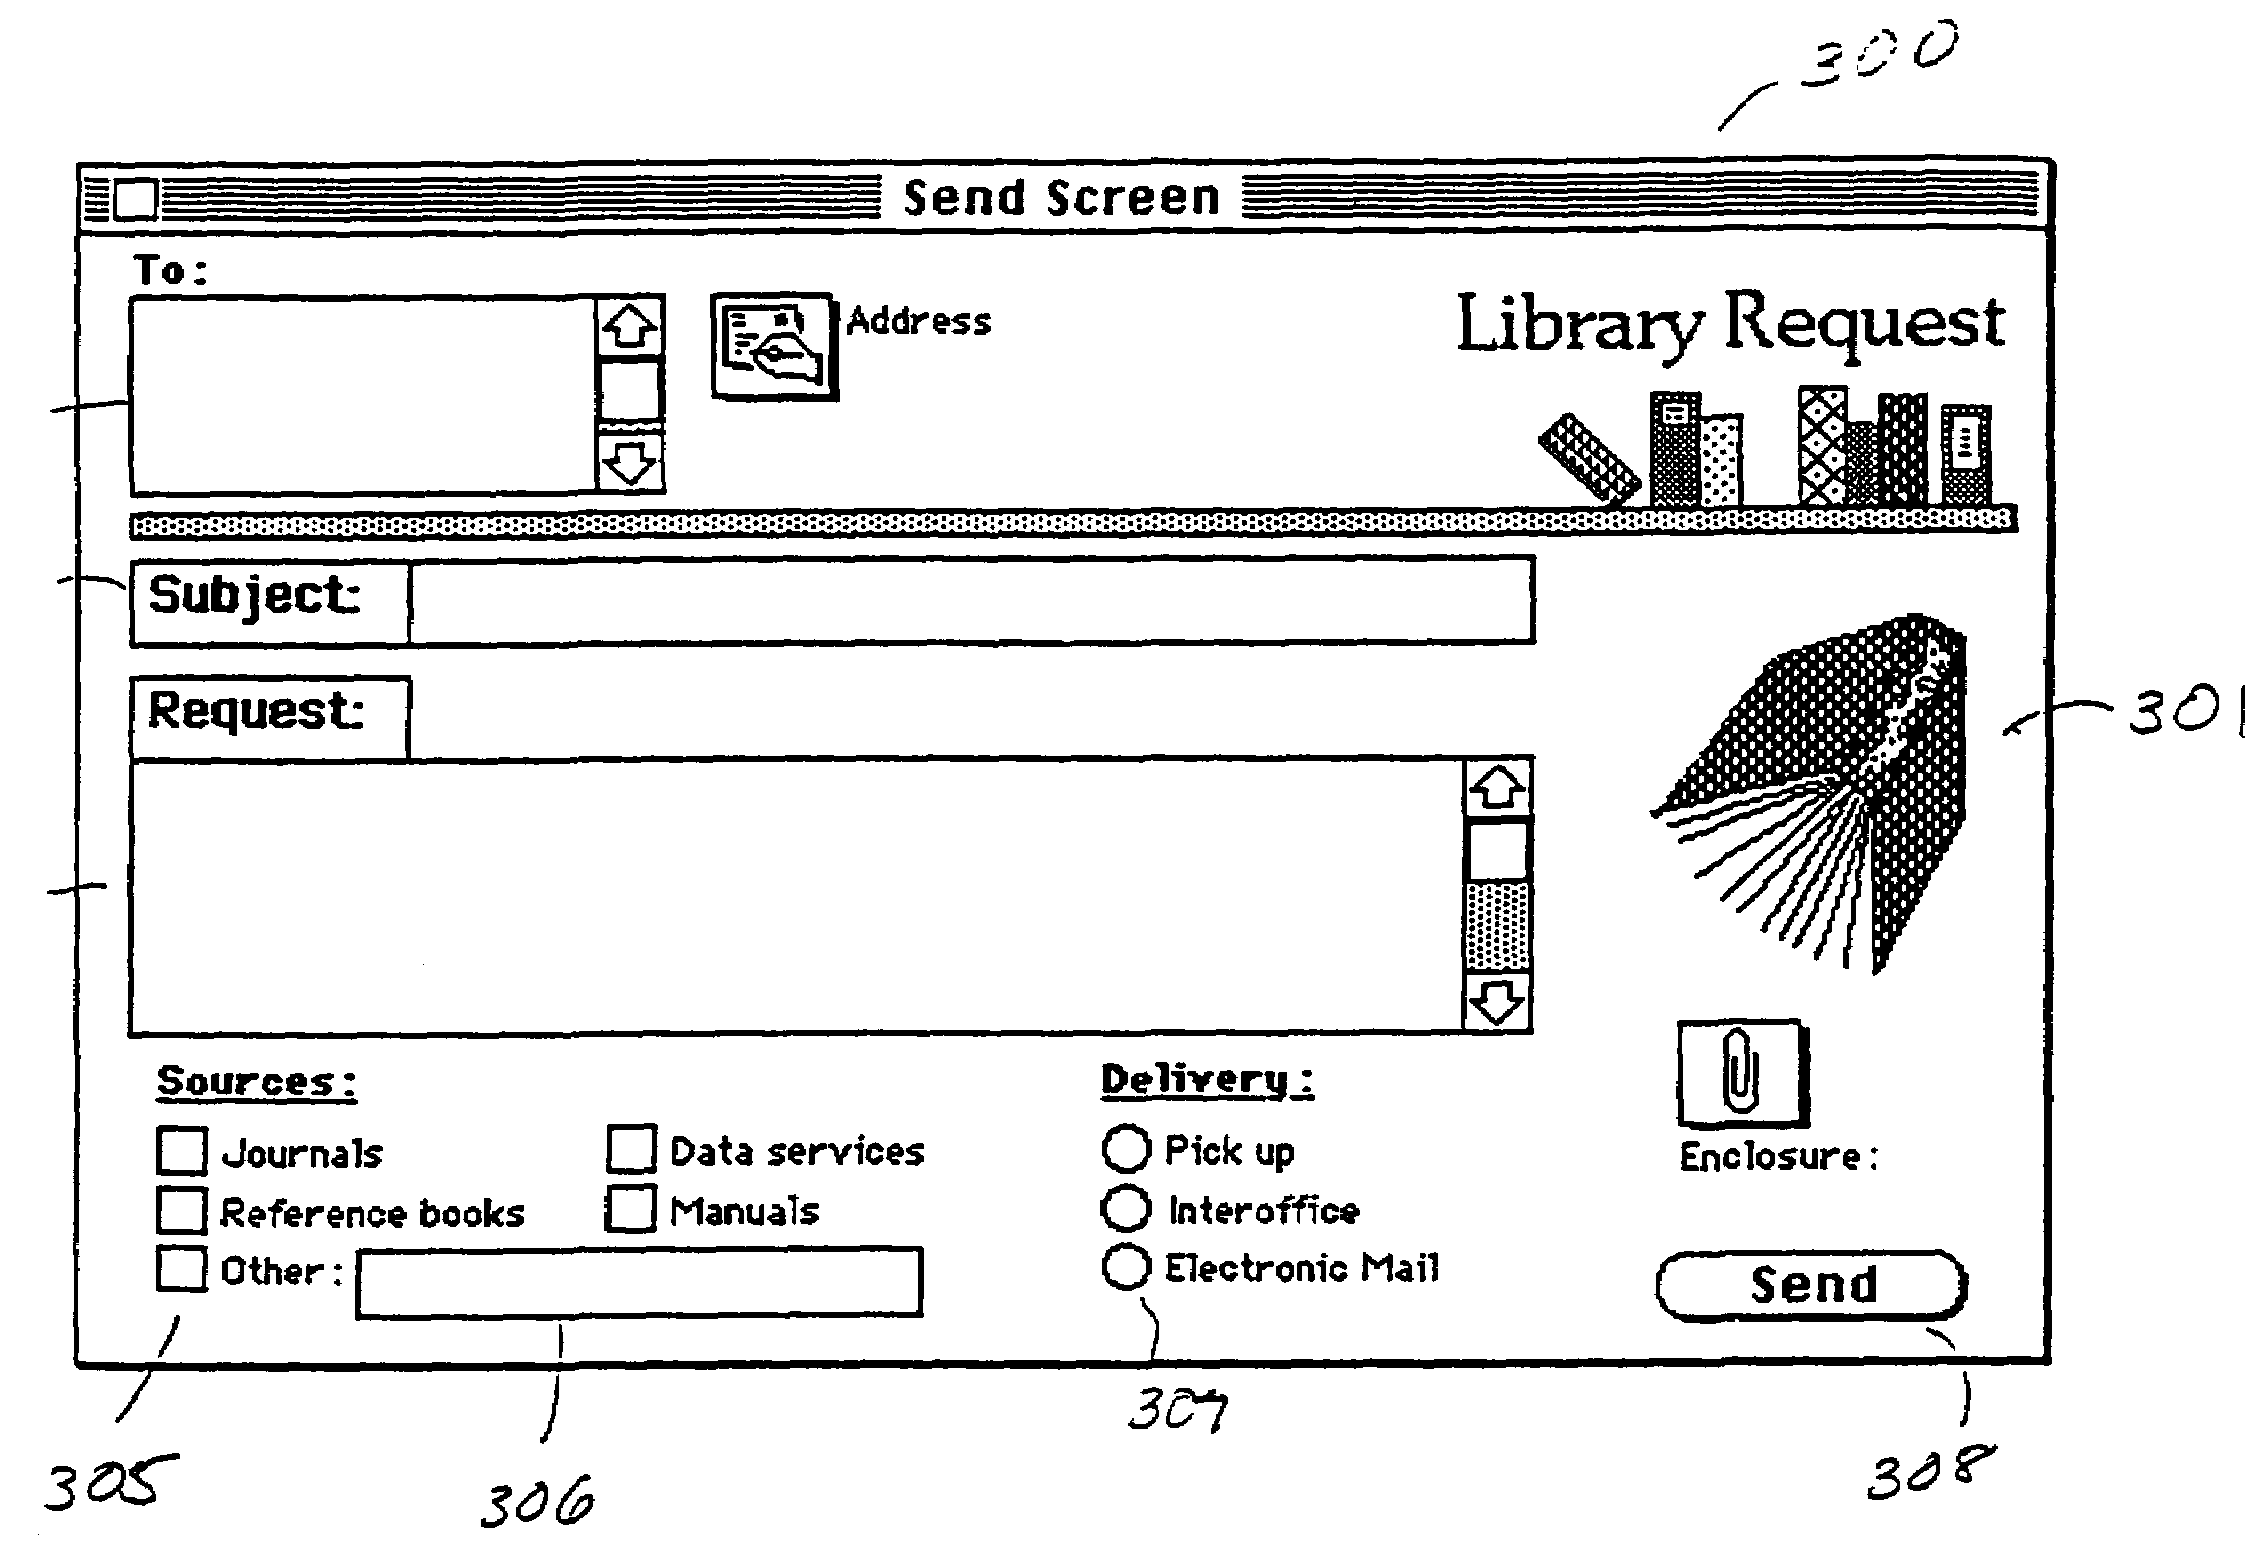
\includegraphics[width=0.7\textwidth]{images/emailform.png}
	\caption{Example Form (Patent \cite{holt_customizing_2006})}
	\label{fig:emailform}
\end{figure}
\end{wrapfigure}

\noindent
a field for address, subject and one for the the actual message to be sent. While an example of what the patent is suggesting can be seen in figure \ref{fig:emailform}, it shows the adding of additional fields allowing for wide variety of form to be created and not limit the  users to use the few forms that are precreated.\\
This increased flexibility in email forms would allow for easier  interpretation of messages, making responding or providing information via email a lot simpler and quicker.


\subsection{Development Tools}
%TODO%

\subsubsection{Jquery}
%TODO%

\subsubsection{Bootstrap}
%TODO%


%%%%%%%%%%%%%%%%%%%%%%%%%%%%%%%%%%%%%%%%%
%										%
%     		 Requirements				%
%										%
%%%%%%%%%%%%%%%%%%%%%%%%%%%%%%%%%%%%%%%%%
\newpage
\section{Requirements}
\label{section:require}
\newcounter{requirement} \stepcounter{requirement}


\subsection{Functional}
Requirements for the system are each given an idea depending on the type of requirement: FR for functional requirements and NFR for non-functional requirements.

Along with this, each requirement has a description stating what the requirement is and a priority. The priority value can be low, medium or high, which shows which requirements will be implemented first into the system.

For this project I will be attempting to implementing all of the high priority functional and nonfunctional requirements, I will also try and implement as many medium and low priority requirements that I can starting with ones that best improve the system.

\def\arraystretch{1.5}
\subsubsection{User Requirements}
Functional requirements also include an access column which defines what users should be able to use. Some items are restricted to lecturers as some requirements should only be be usable by lecturers and lab-helpers and not by students. The table is sorted first by access level starting with widest allowed access then sorted in access order 1 - 4, it is secondly sorted by priority.

The access levels are: 1-Admin, 2-Lecturers, 3-Lab Helpers and 4-Students

\begin{spacing}{1.5}
\begin{longtable}{|p{0.09\linewidth}|p{0.6\linewidth}|p{0.1\linewidth}|
p{0.1\linewidth}|}
\caption{Functional User Requirements} \label{table:funct-user} \\ \hline
\textbf{ID} & \textbf{Requirement} & \textbf{Access} & \textbf{Priority}\\
\hline \hline

\rowcolor{Gray} \rid{FR} & Should have to login to view system & 1,2,3,4 & High\\ \hline
\rid{FR} & Should have accounts created for them & 1,2,3,4 & High\\ \hline
\rid{FR} & Should be able to change password & 1,2,3,4 & High\\ \hline
\rid{FR} & Should be able to login using university ID & 1,2,3,4 & Low\\ \hline
\rid{FR} & Should be able to logout & 1,2,3,4 & High \\ \hline

\rid{FR} & Should be able to remove students from courses & 1, 2 & High\\ \hline
\rid{FR} & Should be able to update student accounts & 1,3 & Low \\ \hline

\rid{FR} & Should be able to look up students in lab & 2,3 & High\\ \hline
\rid{FR} & Should be able  to select students from lab list & 2,3 & High\\ \hline
\rid{FR} & Should be able to leave comments about students & 2,3 & High\\ \hline
\rid{SR} & Should be able to save marks & 2,3 & High\\ \hline
\rid{SR} & Should be able to update marks & 2,3 & High\\ \hline
\rid{SR} & Should be able to delete marks & 2,3 & High\\ \hline
\rid{FR} & Should be able to search for student by name & 2,3 & Medium\\ \hline
\rid{FR} & Should be able to mark student even if they are not in the system & 2,3 & Medium \\ \hline

\rid{FR} & Should be able to assign students to courses & 1 & Medium\\ \hline
\rid{FR} & Should be able to assign lectures to courses & 1 & Medium \\ \hline

\rid{FR} & Should be able to create marking schemes & 2 & High\\ \hline
\rid{FR} & Should display generated stats & 2 & High\\ \hline
\rid{FR} & Should be able to see submitted marks & 2 & High\\ \hline
\rid{FR} & Should be able to generate end of year spread sheets & 2 & Medium\\ \hline
\rid{FR} & Should allow editing of students in class & 2 & Medium\\ \hline
\rid{FR} & Should be able to create peer marking scheme & 2 & Medium\\ \hline
\rid{FR} & Should be able to look at students stats & 2 & Medium\\ \hline
\rid{FR} & Should be able to set what parts of the marking scheme students can see & 2 & Medium\\ \hline
\rid{FR} & Should be able to update marking scheme & 2 & Medium \\ \hline
\rid{FR} & Should be able to delete marking schemes & 2 & Medium\\ \hline
\rid{FR} & Should be able to able to assign students to set labs & 2 & Low \\ \hline
\rid{FR} & Should be able to set penalties for late marking & 2 & Low \\ \hline
\rid{FR} & Should able to export to vision & 2 & Low\\ \hline

\rid{FR} & Should be able to access Marking Scheme & 3 & High\\ \hline
\rid{FR} & Should be able to enter selected students mark & 3 & High\\ \hline
\rid{FR} & Should be able to submit student mark & 3 & High\\ \hline
\rid{FR} & Should be able to select the lab they are helping in & 3 & High\\ \hline

\rid{FR} & Should be able to see current mark & 4 & High\\ \hline

\rid{FR} & Should show different displays depending on access level & & High\\ \hline
\rid{FR} & Should load students current lab mark scheme & & High\\ \hline
\rid{FR} & Should apply penalty for late lab completion & & High\\ \hline
\rid{FR} & Should create a set of useful stats based on lab & & High\\ \hline
\rid{FR} & Should store what class student belong too & & High\\ \hline
\rid{FR} & Should have a list of all students in class & & High\\ \hline

\end{longtable}Each sprint will have set requirements that are to be implemented by the end of the sprint.
\end{spacing}
\setcounter{requirement}{1}


\newpage
\subsection{Non-Functional Requirements}

Table \ref{table:non-func} lists all the non-functional requirements for the development of the system, they are ranked in order of priority.

\begin{spacing}{1.5}
\begin{longtable}{|p{0.1\linewidth}|p{0.7\linewidth}|p{0.1\linewidth}|}
\caption{Non-Function Requirements} \label{table:non-func}\\
\hline
\textbf{ID} & \textbf{Requirement} & \textbf{Priority}\\
\hline \hline


\rid{NFR} & Should have all person data encrypted & High\\ \hline
\rid{NFR} & Should update stats as marks are entered & High\\ \hline
\rid{NFR} & Should take less than 2 seconds to generate stats  & High\\ \hline
\rid{NFR} & PHP Should use prepared statements & High\\ \hline
\rid{NFR} & Should be dynamically designed & High\\ \hline
\rid{NFR} & HTML, CSS and Javascript should be validated & High\\ \hline
\rid{NFR} & Should make sure inputs are valid & High\\ \hline
\rid{NFR} & Should prevent SQL Injection & High\\ \hline


\rid{NFR} & Should function on a wide variety of smart phones and tablets & Medium\\ \hline
\rid{NFR} & Should be able to handle a large number of users without any faults & Medium\\ \hline
\rid{NFR} & Should make sure passwords contain alphanumerics and have a minimum and maximum length  & Medium\\ \hline
\rid{NFR} & Should auto save marks as they are entered & Medium\\ \hline
\rid{NFR} & Should record what lab help marked what student & Medium\\ \hline
\rid{NFR} & Should list all students that did not attend the lab & Medium\\ \hline
\rid{NFR} & Should track how long it takes to mark a student & Medium \\ \hline


\rid{NFR} & Should have disability options (Increase text size, colour layout) & Low\\ \hline
\rid{NFR} & Should be readable by screen readers & Low\\ \hline
\rid{NFR} & Should take less than 2 second to load student marking scheme & Low\\ \hline
\rid{NFR} & Should be able to group marked people & Low \\ \hline
\rid{NFR} & Should retrieve student images from university system & Low\\ \hline
\rid{NFR} & Should backup database regularly & Low\\ \hline


\end{longtable}
\end{spacing}
\setcounter{requirement}{1}


%%%%%%%%%%%%%%%%%%%%%%%%%%%%%%%%%%%%%%%%%
%										%
%     		     Design 				%
%										%
%%%%%%%%%%%%%%%%%%%%%%%%%%%%%%%%%%%%%%%%%
\newpage
\section{Design}
This sections is to explain all the design decision take in developing the marking system using sketches, models and diagrams and thus assist in the understanding of how the system works as a whole. The design aspect that are cover are: the user interface, database design and the main functionality required to make the system work. 

\subsection{User Interface Design}
For the system to be useful the user interface must be easy to use and understand, along with this it will have to be functional on mobile devices as well. To achieve this I have developed mock-ups for main web pages required to make the system work, including a design for desktop and mobile. 

\subsubsection{Lab Results}
%TODO%
\subsubsection{Lab Maker}
%TODO%
\subsubsection{Marking}
%TODO%
\subsubsection{Lab Creation}
%TODO%

\subsection{Database Design}
%TODO%

\subsection{Functionality Design}
%TODO%



%%%%%%%%%%%%%%%%%%%%%%%%%%%%%%%%%%%%%%%%%
%										%
%     		 Implementation				%
%										%
%%%%%%%%%%%%%%%%%%%%%%%%%%%%%%%%%%%%%%%%%
\newpage
\section{Implementation}
%TODO%

\subsection{Database}

\subsection{Lab Creator}
%TODO%

\subsection{Marking Labs}
%TODO%

\subsection{Results Display}
%TODO%
\subsubsection{Students}
%TODO%
\subsubsection{Lecturers}
%TODO%

\subsection{Lab Management}
%TODO%

\subsection{Admin Panel}
%TODO%





%%%%%%%%%%%%%%%%%%%%%%%%%%%%%%%%%%%%%%%%%
%										%
%     		Testing & Evaluation		%
%										%
%%%%%%%%%%%%%%%%%%%%%%%%%%%%%%%%%%%%%%%%%
\newpage
\section{Strategy for testing and evaluation}

\subsection{Testing}
%TODO%
\subsubsection{Development Testing}
%TODO
\subsubsection{Final Testing}
%TODO


\subsection{Evaluation}


\subsubsection{Usability Case Study}
%TODO
\subsubsection{Feedback}
%TODO%
\subsubsection{Implementation Of Feedback}

%%%%%%%%%%%%%%%%%%%%%%%%%%%%%%%%%%%%%%%%%
%										%
%     	       Discussion				%
%										%
%%%%%%%%%%%%%%%%%%%%%%%%%%%%%%%%%%%%%%%%%
\newpage
\section{Discussion}
%TODO%

\subsection{Development}
%TODO%

\subsection{Limitations}
%TODO%

\subsection{Future Improvements}
The electronic marking system has many improvements that can be implemented some are requirements that I was not able to implement 

\subsection{Conclusion}
%TODO%


%%%%%%%%%%%%%%%%%%%%%%%%%%%%%%%%%%%%%%%%%
%										%
%     		Bibliography				%
%										%
%%%%%%%%%%%%%%%%%%%%%%%%%%%%%%%%%%%%%%%%%


\newpage
\printbibliography[heading=bibintoc]
\let\cleardoublepage\clearpage


%%%%%%%%%%%%%%%%%%%%%%%%%%%%%%%%%%%%%%%%%
%										%
%     		Appendices					%
%										%
%%%%%%%%%%%%%%%%%%%%%%%%%%%%%%%%%%%%%%%%%


\begin{appendices}

\let\cleardoublepage\clearpage

\end{appendices}

\end{document}